\

\vfill

\begin{center}
    \begin{quotation}
    \raggedleft
    \textit{The more complex a system is, the more \newline difficult its correctness verification will be.}
    \end{quotation}
\end{center}
\vfill

\chapter{Introduction to Cybersecurity}


\section{Risk Estimation and Management}
\cite{01_introduction}
Complexity is an enemy of security, in fact, consequence of a succsseful attack are as follows:
\begin{itemize}
    \item \textbf{Financial loss}: Successful cyberattacks can result in significant financial damages, whether through direct theft, fraud, or the cost of mitigating the attack. These costs may include legal fees, regulatory fines, and compensation for affected parties, further impacting the financial stability of the organization.
    \item \textbf{Recovery Cost}: After a cyberattack, the cost of recovering data, restoring systems, and rebuilding infrastructure can be astronomical. This includes expenses for forensic investigations, IT support, and additional security measures to prevent future incidents. Recovery can take weeks, months, or even longer, depending on the extent of the damage.

\item \textbf{Productivity Loss}: Cyberattacks often lead to downtime as systems are taken offline for repairs, investigation, or containment. Employees may be unable to access necessary resources, leading to decreased efficiency, missed deadlines, and slower response times. The longer the recovery process, the greater the impact on business operations.

\item \textbf{Business Disruption}: Attacks such as Distributed Denial of Service (DDoS) or ransomware can completely halt business operations, making it impossible for customers to access services or for employees to perform essential tasks. This disruption can result in lost revenue, delayed projects, and long-term operational inefficiencies.

\item \textbf{Reputation Damage}: The fallout from a cyberattack can severely damage an organization's reputation, leading to a loss of customer trust. Once confidential data is compromised or service outages occur, customers may feel their information is not secure, causing them to take their business elsewhere. In some cases, the reputational damage can take years to repair, even if the security breach is fully addressed.
\end{itemize}

\clearpage

\begin{multicols}{2}
    Terminolgy:
    \begin{itemize}
        \item Asset: the set of goods, data and people needed for an IT service.
        \item Vulnerability: intrinsic weakness of an asset.
        \item Threat: possible deliberate action/accidental event that can produce the loss of a security property by exploiting a vulnerability.
        \item Attack: threat occurrence (deliberate action)
        \item (Negative) event: threat occurrence (accidental event)
    \end{itemize}
    \columnbreak
    
    \begin{figure}[H]
        \centering
        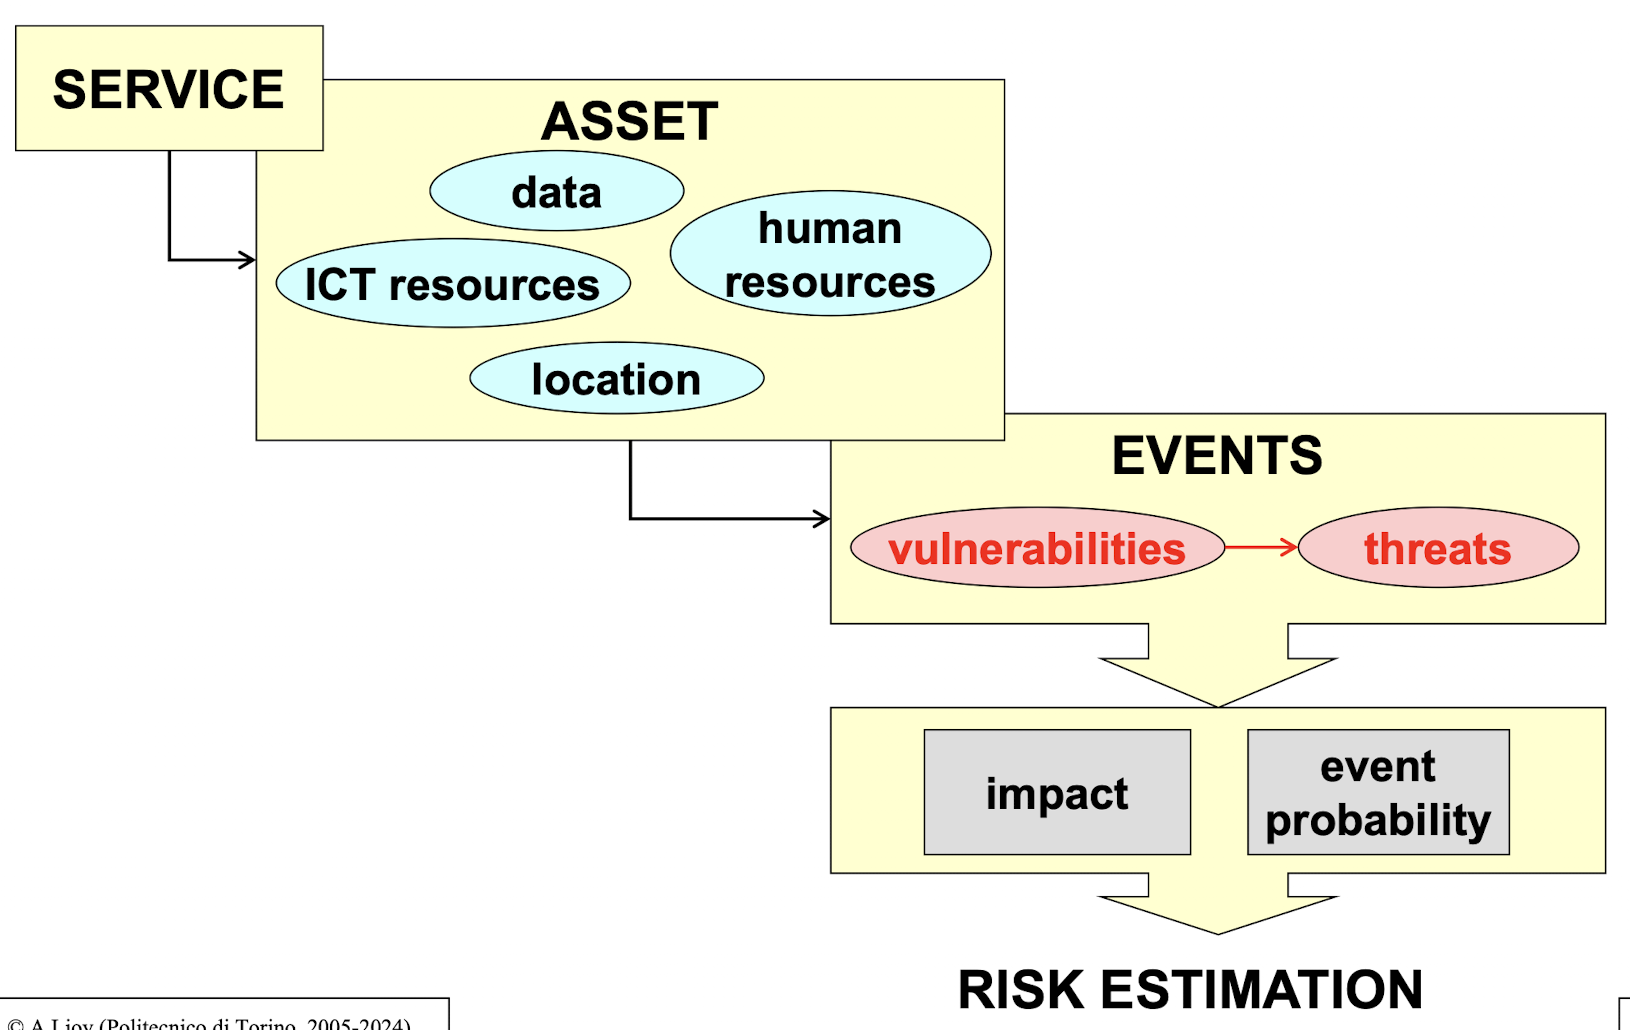
\includegraphics[width=\linewidth]{Images/Introduction/riskEvaluation.png}
        \caption{The risk estimation process}
    \end{figure}
\end{multicols}

Managing threats requires us to \textbf{prioritize risks}, considering not only the impact but also the available \textbf{time and budget}\footnote{A risk assessment matrix (or risk heat map) can be useful in this process}.

\begin{figure}[H]
    \centering
    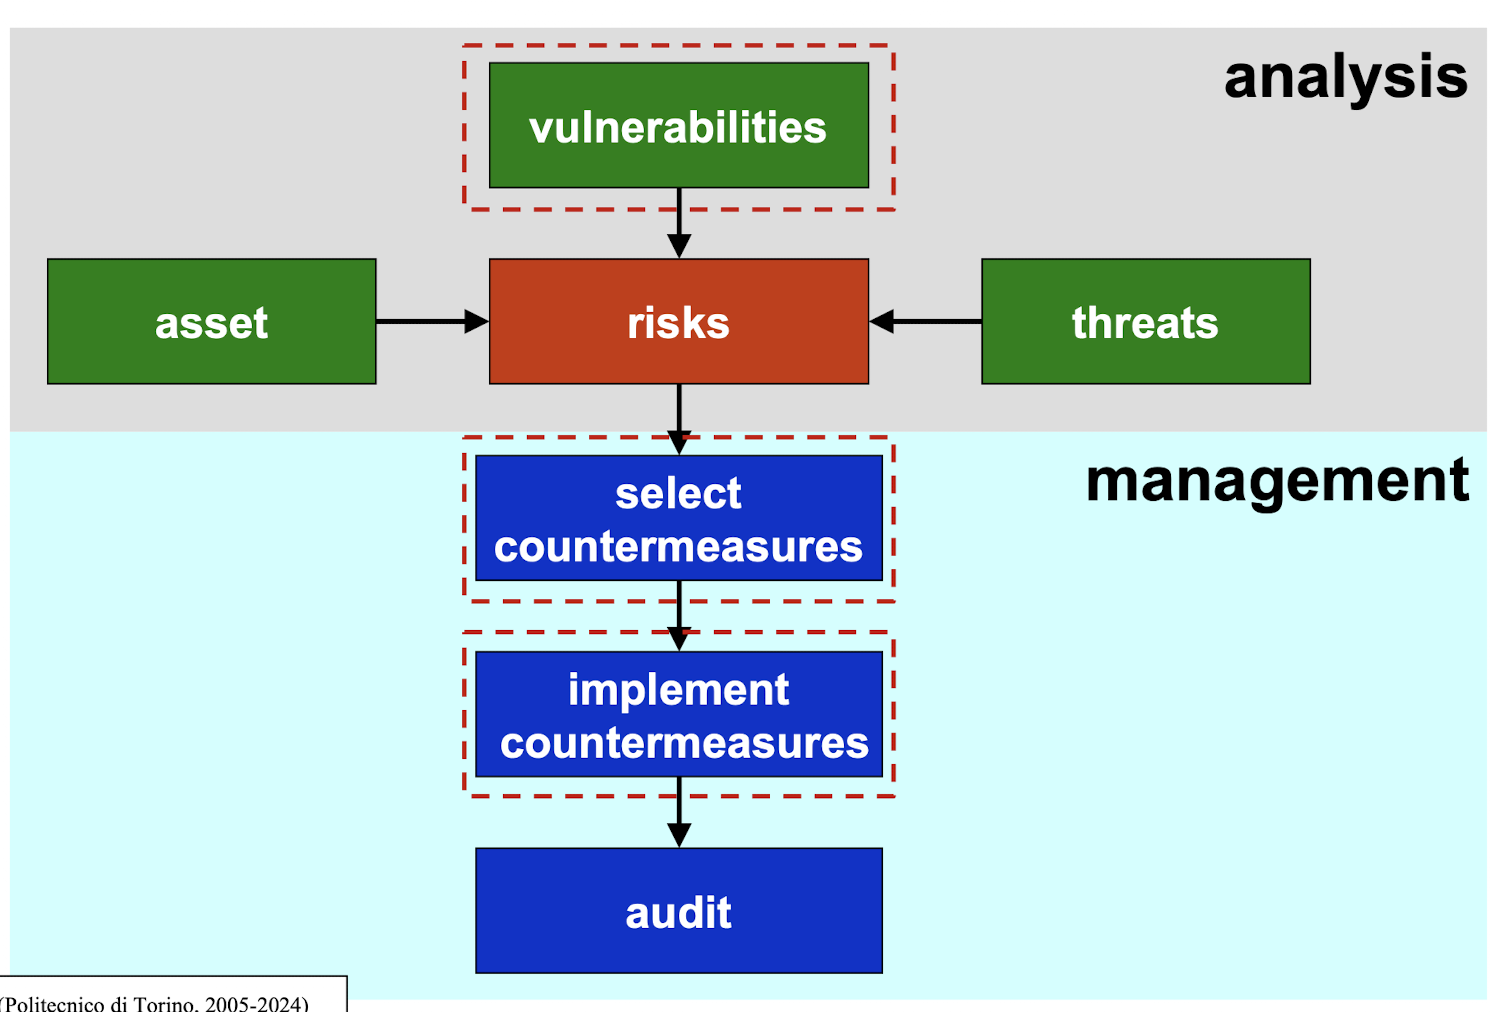
\includegraphics[width=0.5\linewidth]{Images/Introduction/analysisAndManagement.png}
    \caption{Analysis and management of security}
\end{figure}

\subsection{Data Protection}
For each security property always consider the three cases of data protection: data in transit (protected channel), data at rest (protected disk) and data at work (protected memory).

\subsection{Threat Model}
An enemy performs actions based on its position and capabilities. When considering attacks from a positional perspective, we can distinguish between different types of attack vectors: Man In The Middle (MITM), Man At The End (MATE), Man In The Browser (MITB). On the other hand capabilities influence the attack methods and level of sophistication the enemy can employ. For instance, an enemy can act as a passive attacker, merely reading data or traffic without altering it, or as an active attacker, who not only reads but also modifies or injects data into the traffic.

\subsection{Basic Problems}
Modern networks face several technological vulnerabilities that make them susceptible to various security threats. Firstly, network communications are often insecure. Many communications are transmitted in plain text, making them easy to intercept. Additionally, LANs typically operate in broadcast mode, which exposes data to anyone within range, and wireless communications are similarly vulnerable to interception due to the lack of encryption. Geographic connections between locations do not use end-to-end dedicated lines; instead, they rely on shared lines and third-party routers, further compromising security.

Another major issue lies in authentication practices. User authentication mechanisms are generally weak, as they are usually password-based, which is insufficient for robust security. Furthermore, server authentication is often either non-existent or poorly implemented, leaving servers open to unauthorized access.

Lastly, the software running on these networks tends to have numerous bugs. These vulnerabilities can be exploited by attackers, further undermining the security of the system. Addressing these fundamental issues is critical to improving network security and protecting sensitive information.

Non-technological problems in cybersecurity often stem from human factors and system design issues. One major challenge is low problem understanding or awareness; many users are unaware of the risks and threats they face online, which makes them vulnerable to attacks. Additionally, human error plays a significant role, especially when individuals are overloaded, stressed, or distracted, leading to mistakes such as falling for phishing scams or misconfiguring security settings. Another issue is that human beings have a natural tendency to trust systems and people, which cyberattackers can exploit through social engineering tactics like phishing or pretexting. Moreover, complex interfaces and architectures can mislead users, making it harder for them to identify potential security threats or navigate security features correctly. This can result in inadvertent errors, such as incorrect file permissions or failure to apply security patches.

Lastly, performance decreases due to the application of security measures can discourage users from fully implementing necessary protections, as they may prioritize convenience or speed over safety. These non-technological factors are critical in understanding how cybersecurity vulnerabilities can arise and emphasize the need for user education, simplified interfaces, and effective security practices.

\hfill 
\begin{center}
    Refer to Appendices A and B for a clearer understanding of potential attacks and attack vectors.
\end{center}
\hfill

\subsection{NIST Cybersecurity Framework}
The NIST Cybersecurity Framework is a set of guidelines developed by the National Institute of Standards and Technology (NIST) to help organizations manage and mitigate cybersecurity risks. It provides a flexible, risk-based approach to cybersecurity and is widely used across various industries. The framework is structured around five core functions, which are designed to be applied in a continuous cycle:
\begin{itemize}
    \item Identify: Develop an understanding of the organization’s cybersecurity risks by identifying assets, vulnerabilities, threats, and impacts. This includes understanding business objectives, resources, and risk tolerance.
    \item Protect: Implement safeguards to ensure the delivery of critical infrastructure services. This includes access control, data security, awareness programs, and protective technologies to limit cybersecurity risks.
    \item Detect: Implement monitoring systems to identify cybersecurity incidents. This function involves continuous monitoring for anomalies, events, and potential breaches.
    \item Respond: Develop and implement an action plan for responding to detected cybersecurity incidents. This involves planning and coordination for incident management and mitigation strategies.
    \item Recover: Develop and implement strategies to restore capabilities or services that were impacted by a cybersecurity incident. This ensures that recovery processes are in place for business continuity.
\end{itemize}

\begin{figure}[H]
    \centering
    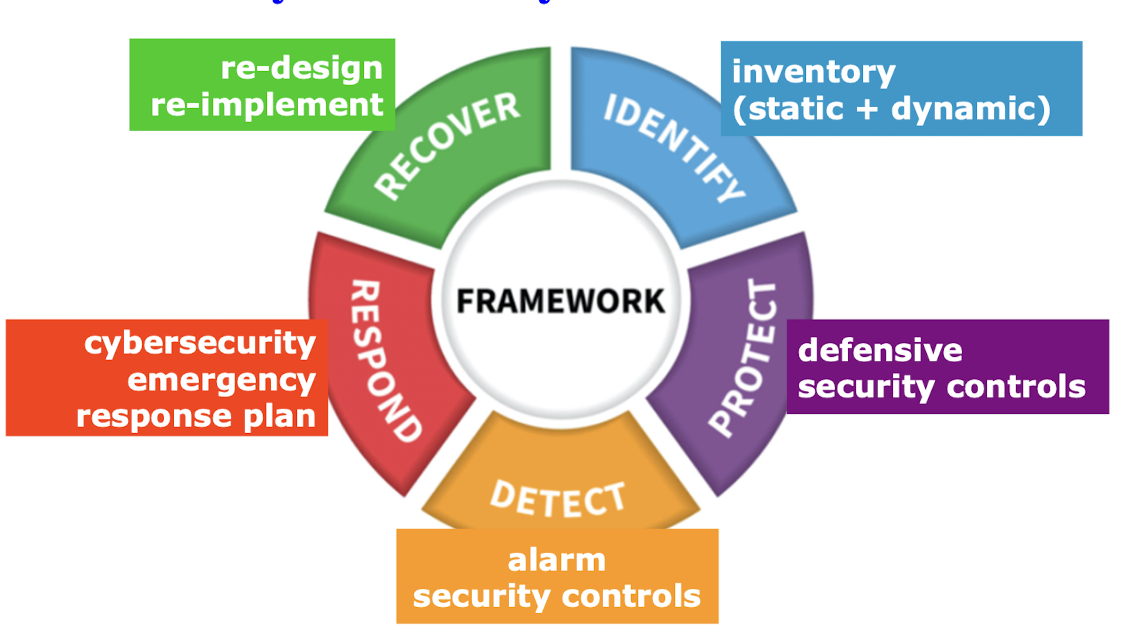
\includegraphics[width=0.5\linewidth]{Images/Introduction/nistFramework.png}
    \caption{NIST cybersecurity framework}
\end{figure}